%%%%%%%%%%%%%%%%%%%%%%%%%%%%%%%%%%%%%%%%%%%%%%%%%%%%%%%%%%%%%%%%%%%%%%%%%%%
%%%                         Metodologia                                 %%%
%%%%%%%%%%%%%%%%%%%%%%%%%%%%%%%%%%%%%%%%%%%%%%%%%%%%%%%%%%%%%%%%%%%%%%%%%%%

\chapter{Metodologia}
\label{ch:metodologia}

Uma pesquisa qualitativa é descrita por \cite{yin2016pesquisa} como uma
investigação com capacidade de entender, traduzir e valorizar as visões dos
sujeitos envolvidos diretamente no fenômeno estudado. É capturar as perspectiva
dos participantes.

Nesse sentido, a pesquisa caracteriza-se pelo caráter qualitativo, pois foca nos
significados e nas percepções de professores e alunos ao longo da intervenção
pedagógica. 

É fundamental abranger dimensões sociais, institucionais e ambientais, nas quais
a vida humana se desenrola. Esses fatores exercem profunda influência sobre os
comportamentos e eventos investigados.\cite{yin2016pesquisa}. 

A metodologia Design-Based Research (DBR), amplamente utilizada na criação de
práticas educacionais, serve como base para o desenvolvimento deste estudo. Essa
metodologia oferece uma estrutura que permite a elaboração de artefatos
pedagógicos dirigidos à intervenção e solução de problemas no âmbito
educacional. Tendo em vista que o propósito deste anteprojeto de pesquisa é
estruturar o desenvolvimento de um sistema para contextos educacionais, a DBR se
estabelece como o fundamento deste estudo.

A DBR é definido por \cite{plomp2018pesquisa} como uma abordagem colaborativa e
iterativa ou uma família de abordagens de pesquisa, não apenas como metodologia
estrita. Fundamenta-se em aspectos como projetar e produzir soluções no contexto
educacional e aprofundar o conhecimento científico sobre essas intervenções,
criando alicerce teórico ou princípios de design e gerar futuras aplicações.

De acordo com \cite{plomp2018pesquisa}, essas intervenções dirigidas à resolução
de problemas práticos não se limitam a mudanças curriculares, abrangendo
explicitamente a formulação de artefatos pedagógicos, materiais, produtos e
sistemas voltados para a educação. É pragmática, intervencionista e
colaborativa, pois pesquisadores e profissionais da educação podem trabalhar
juntos.

\begin{citacao}
    intervencionista: a pesquisa objetiva a elaboração de uma intervenção para
    uma situação da vida real [...] envolvimento dos praticantes: a pesquisa
    envolve a participação ativa ou a colaboração com os praticantes em vários
    estágios e atividades da pesquisa — isto aumenta a chance de que a
    intervenção se torne, de fato, relevante e prática para o contexto
    educacional [...] O design é caracterizado por sua ênfase nas soluções,
    guiadas por propósitos mais amplos e metas ideais. Além disso, o design
    desenvolve e projeta propostas que são testadas em experimentos pragmáticos
    e fundamentadas na ciência educacional [...] \cite{obrien2018practical}
\end{citacao}

A DBR define fases que consistem em identificar o problema, propor o
desenvolvimento de soluções, ciclos de aplicação e refinamento iterativos. Por
fim, reflexões e melhorias.

O fluxo a seguir descreve as etapas e as estratégias empregadas para o
desenvolvimento da intervenção.

\begin{figure}[H]
    \centering
    \caption{Fluxo geral do DBR}
    \label{fig:fluxo-geral-dbr}
    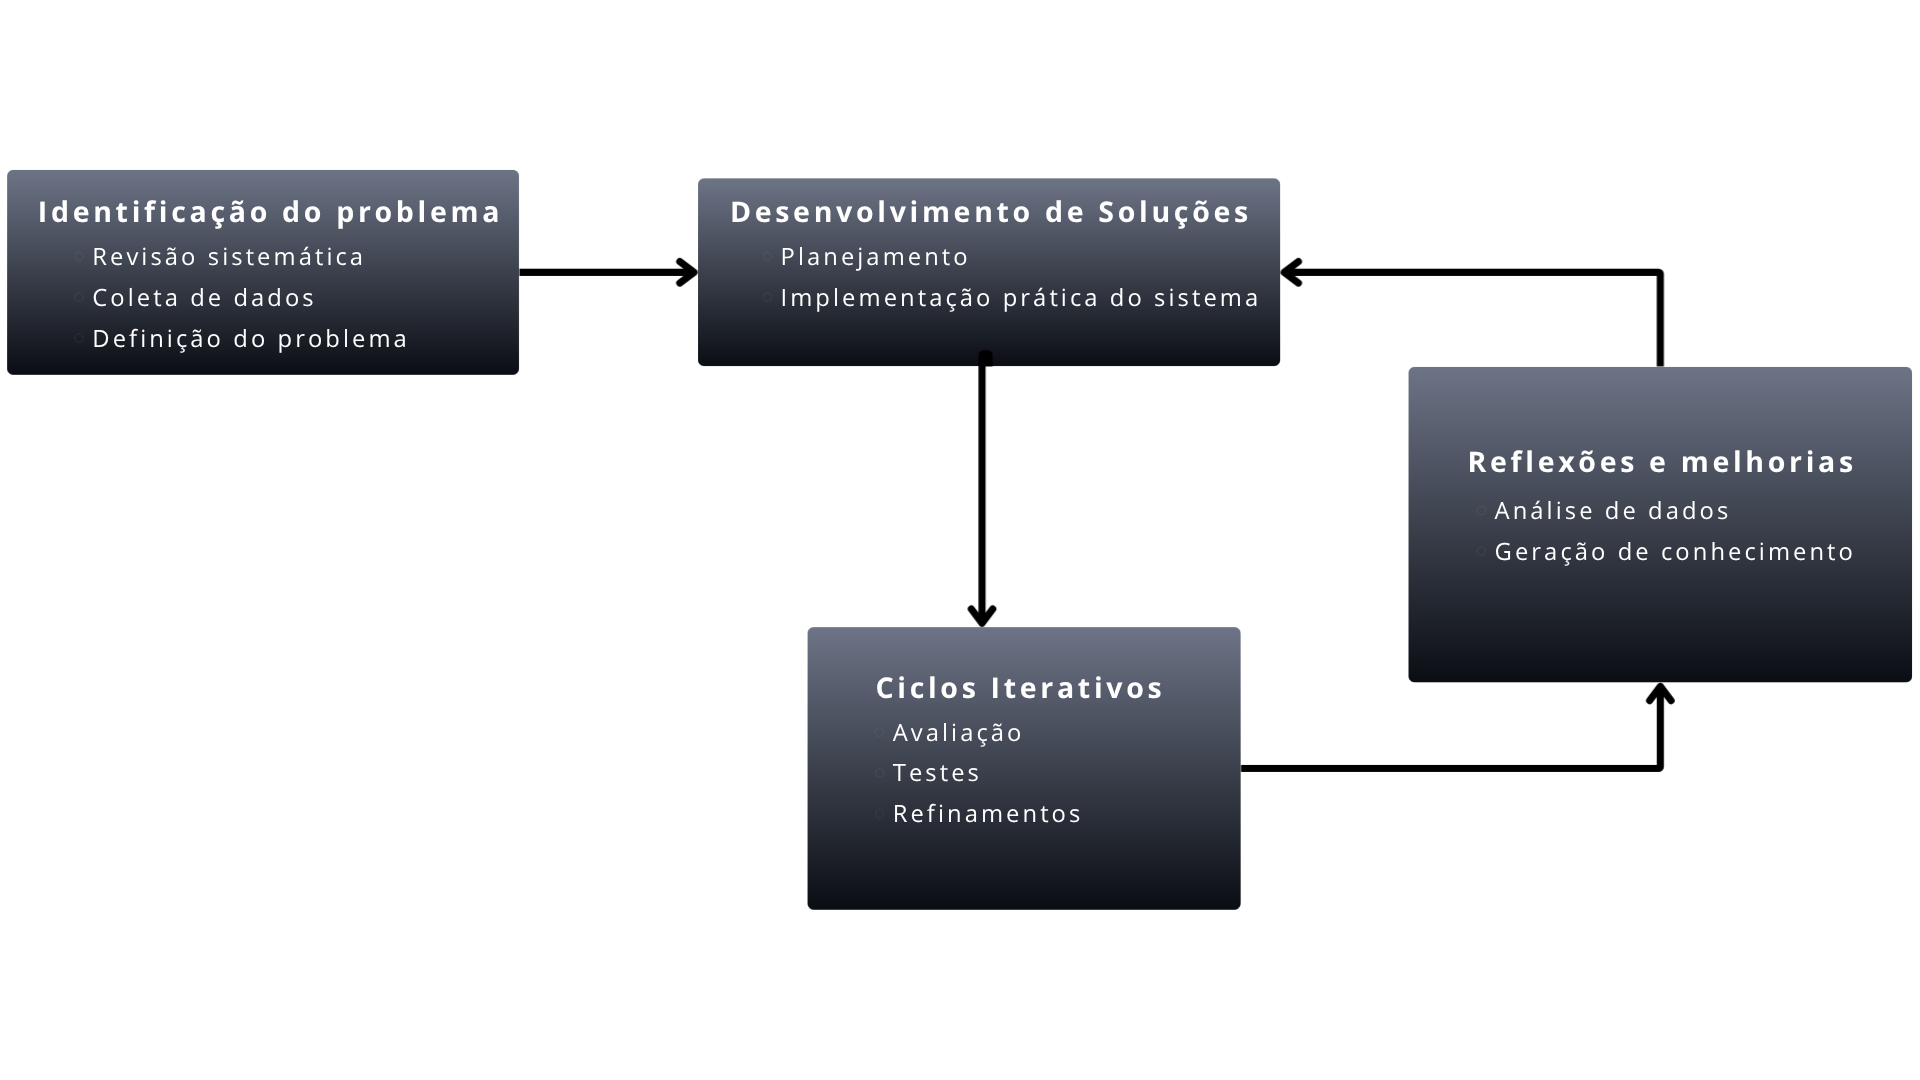
\includegraphics[width=\textwidth]{figuras/Fluxo_Geral_DBR.png}
    \fonte{Elaborado pelo autor (2026).}
\end{figure}

A operacionalização da pesquisa encontra-se na tabela abaixo, que correlaciona
as fases conceituais da (DBR) com os entregáveis do desenvolvimento do projeto.

\renewcommand{\tablename}{Quadro}
\renewcommand{\arraystretch}{1.5} 
\begin{longtable}{ | >{\bfseries\raggedright\arraybackslash}p{4.0cm} |
    >{\raggedright\arraybackslash}p{10.5cm} |} \caption{Etapas do DBR e seus
    respectivos desenvolvimentos} \label{quadro:dbr} \\
    \hline
    \normalfont\bfseries Etapas do DBR & \normalfont\bfseries Etapas de
    Desenvolvimento \\
    \hline    \endhead
 
    Identificação do problema & Revisão Sistemática de Literatura. Mapear as
    principais competências matemáticas das questões do ENEM e como o PC é desenvolvido. \\
    \hline
 
    Desenvolvimento de soluções & Definição da arquitetura e das mecânicas de
    gamificação da plataforma. Desenvolvimento da primeira versão funcional da
    plataforma. \\
    \hline
 
    Ciclos iterativos & Ciclo 1:Avaliação por professores de Matemática do curso
    de Sistemas de Informação. Ciclo 2: Avaliação por alunos da UPT.\\
    \hline
 
    Reflexões e melhorias & Ciclo 1: Refinamento do sistema a partir do feedback
    dos professores. Ciclo 2: Uso de sistema pelos alunos e aplicação dos
    formulários ESM e UES. Analisar os dados dos formulários e geração de
    conhecimento. \\
    \hline
\end{longtable}

\begin{center}
    \vspace{-0.5cm}
    {\small Fonte: Elaborado pelo autor (2026).}
\end{center}

\section{Identificação do problema}
\sloppy

A etapa inicial da metodologia DBR é a investigação preliminar, descrito por
\cite{obrien2018practical}, como parte essencial para obter um insight profundo
sobre o problema educacional, compreendendo a situação-problema e as
possibilidades de inovação. Em relação ao referencial teórico, a revisão
sistemática de literatura implementada formaliza esse processo, explorando bases
de conhecimento, avaliando intervenções ou projetos sobre a temática do
Pensamento Computacional e gamificação para o contexto da aprendizagem em
matemática. O contexto do problema consiste em argumentar sobre o baixo
desempenho em matemática no ENEM e a falta de práticas voltadas para o tema.

\section{Ciclos Iterativos de Avaliação}
Os ciclos iterativos e de avaliação, de acordo com \cite{obrien2018practical}
são testes e refinamentos das soluções. Esse processo, na prática, é repetido
até que alcance um equilíbrio entre o que foi idealizado e a produção. É feito
uma avaliação formativa a cada ciclo, pois é o motor que impulsiona o avanço.

A etapa de ciclos iterativos é dividida em duas etapas: Ciclos de validação por
especialistas e aplicação com alunos.
\subsection{Ciclo de validação por especialistas}

Grupo focal é descrito por \cite{gil2021pesquisa} como um tipo especial de grupo
em termos de finalidade, tamanho, composição e procedimentos. Um grupo focal não
busca consenso, mas encoraja a expressão de respostas que possibilitam uma
melhor compreensão das atitudes, comportamentos, opiniões e percepções dos
participantes. Caracteriza-se pelo uso explícito da interação para gerar dados.

Segundo \cite{gil2021pesquisa}, o planejamento do grupo focal é uma das
estratégias mais estruturadas entre as variadas abordagens empregadas na coleta
de dados em pesquisas qualitativas, exigindo que o pesquisador faça uma série de
decisões rigorosas. Os participantes devem estar em consonância com os objetivos
da pesquisa.

O grupo focal será composto pelos especialistas em matemática do curso de
Sistemas de Informação, uma vez que a experiência dos professores os torna aptos
para avaliar a viabilidade pedagógica do sistema.

Validação com professores de matemática do curso de Sistemas De Informação,
focando no \textit{feedback}. Segundo \cite{plomp2018pesquisa} descreve que o
protótipo deve ser submetido a revisões e refinamentos a partir da avaliação dos
especialistas, para que as intervenções educacionais ultrapassem a idealização
teórica, e que sua aplicabilidade e sua capacidade de sobreviver e funcionar de
maneira efetiva frente às condições, desafios e restrições reais do contexto
educacional e do "chão da escola".

A avaliação do sistema por parte dos professores será conduzida com foco na
validação dos conteúdos matemáticos, verificando se os enunciados, dados e
gabaritos mantêm a acurácia e o rigor conceitual exigidos. Como o sistema trata
e processa essas demandas cognitivas e se as mecânicas de gamificação foram
projetados de modo a induzir e estimular o raciocínio. 

\subsection{Ciclo de validação por alunos}
Os ciclos de validação pelos alunos tem como objetivo aferir se o produto
resultou nos impactos e nas consequências de aprendizagem desejados e como a
intervenção afeta o raciocínio, compreensão, criatividade, atitude e a motivação
dos alunos, como descrito por \cite{plomp2018pesquisa}.

Nessa etapa serão aplicados os formulários de Método de Amostragem de
Experiência (ESM) e Escala de Engajamento do Usuário (UES).

\subsubsection{Método de Amostragem de Experiência (ESM)}
O método de amostragem de experiência é utilizado para medir a experiência do
usuário ao utilizar um sistema, coletando informações durante o uso. É descrito
por \cite{francisco2020esm}, como investigações que necessitam coletar dados de
uma experiência que ocorreu com base em um evento específico para entender como
os participantes interagem com o sistema.

O uso desse método fundamenta-se na necessidade de garantir a adesão dos
participantes, pois os usuários são mais dispostos a responder quando o
questionário é curto, simples, fácil de compreender e responder, não exigindo
muito esforço mental \cite{francisco2020esm}.

A aplicação do método consiste na criação do formulário de amostragem da
experiência do usuário, utilizando a Escala Likert com campos de resposta com
radio buttons, checkboxes e campos abertos. 

De acordo com \cite{francisco2020esm}, a criação do formulário deve considerer a
possibilidade de resposta em menos de um minuto. A agilidade deve ser garantida
por meio de campos de resposta rápida. Quando o objetivo for medir o grau de
concordância com uma afirmação, deve-se preferir o uso de escalas menores, como
a de 5 pontos, visto que escalas maiores fazem o participante parar para pensar.
Por outro lado, os campos abertos devem ser evitados ou minimizados ao máximo,
pois podem tornar a entrada de dados cansativa.

Por fim, \cite{francisco2020esm} destaca que o sucesso da coleta depende de uma
configuração técnica voltada para o imediatismo da emoção sentida no jogo.
Estabelecer esse limite máximo de tempo para o preenchimento é essencial a fim
de garantir que o dado coletado reflita a experiência do momento e não após a
sua ocorrência.

\subsubsection{Escala de Engajamento do Usuário (UES)}
A escala de engajamento do usuário é o critério para medição do engajamento e é
divido em dimensões, descrito por \cite{obrien2018practical}, que estabelece o
instrumento de medição composto por doze questões e quatro dimensões
estruturais: Atenção Focada, Usabilidade Percebida, Apelo Estético e Recompensa.

Segundo \cite{obrien2018practical} a atenção focada reflete estado em que o
indivíduo se sente pela experiência interativa. A usabilidade percebida envolve
a relação entre nível de esforço, sendo a percepção do nível de controle e a
quantidade de esforço que o usuário precisa investir para realizar sua tarefa. O
apelo estético avalia o nível de atratividade e o apelo visual proporcionados
pela interface. 

A dimensão referente a recompensa caracteriza-se pelos aspectos do resultado
experiencial, consolidando sucesso geral da interação e a disposição do usuário
em recomendar o sistema (durabilidade), o interesse e a curiosidade despertados
durante o uso (novidade), além da sensação lúdica de ter se divertido e sido
atraído pela experiência (envolvimento sentido) \cite{obrien2018practical}.

No formulário é usado a Escala de Likert como instrumento de medição do nível de
concordância das respostas. Nessa avaliação, o participante deve refletir sobre
a sua experiência com o sistema e selecionar um valor que varia de 1 (Discordo
Totalmente) até 5 (Concordo Totalmente) para cada item.

Conforme \cite{obrien2018practical}, durante a aplicação do instrumento de
avaliação, o participante deve refletir acerca de sua experiência interativa com
o sistema e indicar seu nível de concordância para cada afirmação.

Em relação ao processo de aplicação do formulário, \cite{obrien2018practical}
destaca que a aplicação do formulário deve ser apresentado de maneira misturada
e aleatória, sendo estritamente necessário que os identificadores originais das
dimensões fiquem ocultos ao respondente. 
\newpage
No momento da apuração dos resultados para o cálculo de fato, os autores
ressaltam que o passo primário e obrigatório é realizar a inversão das notas
(método de reverse code) das questões negativas pertencentes à Usabilidade
Percebida.

\begin{citacao}
Inverta a codificação dos seguintes itens: PU-S1, PU-S2, PU-S3. [...] As
pontuações para cada uma das quatro subescalas podem ser calculadas somando os
valores das respostas para os três itens contidos em cada subescala e dividindo
por três. [...] Uma pontuação geral de engajamento pode ser calculada somando
todos os itens juntos e dividindo por doze \cite{obrien2018practical}
\end{citacao}

Por fim, a pontuação específica de cada subescala é extraída a partir da média
aritmética simples, enquanto o escore do engajamento geral do indivíduo é obtido
pela soma de todas as doze respostas finais da avaliação.

